\section{Semantic Web}

The Semantic Web (SW) is the World Wide Web extension  that  provides a common framework to share and reuse data across application, enterprise, and community boundaries. Tim Berners-Lee, the inventor of the World Wide Web and director of the World Wide Web Consortium (W3C), supervises the development of proposed Semantic Web standards, which is collaborative effort led by W3C with participation from a large number of researchers and industrial partners. 

"The Web can reach its full potential if it becomes a place where data can be processed by automated tools as well as people". [W3C, 2001]

In vision the Semantic Web, in the Web 3.0 the information can be processed and manipulated by machines. SW can give to the information a well defined meaning by adding a new layer of meta-data to the existing documents and data. The semantic definition of data and documents enable to understand and respond to complex human needs. The outcome of this vision is the evolution to a new where intelligent agents can browse data on behalf of the user and make knowledge easier to be reached.


\begin{figure}[tbh]
  \centering
	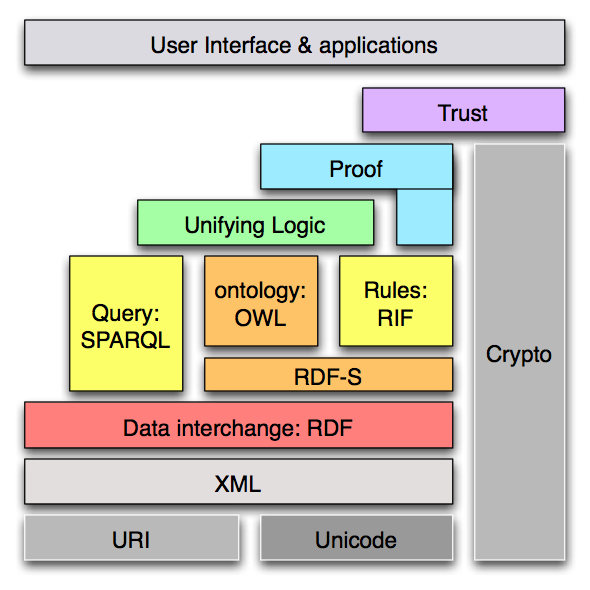
\includegraphics[width=0.75\linewidth]{images/semantic_web_stack}
	\caption{Semantic Web Stack} 
  	\label{fig:semantic-web-stack}
\end{figure}
 

Semantic Web world involved several technologies. Due to the complexity of the concept, the W3C proposed a layered  approach, in which each level contains a set of standards for semantic technologies:

Figure \ref{fig:semantic-web-stack} shows this structure.

At the  On the top of them, the basic syntax level is provided by the eXtensible Markup Language (XML), a wide-spread standard for data exchange in the Web. The XML parsers support the lower-level syntax checking of the Semantic Web documents. However, the XML standard alone is not enough for the data exchange in the semantic web, because it is suited to recognize syntax, but not equivalent models.

The first two level of the Semantic Web stack in Figure \ref{fig:semantic-web-stack} includes some standard of World Wide Web:
\begin{itemize}
\item  The Uniform Resource Identifier (URI)  and Internationalized Resource Identifier(IRI), which guarantee the interoperability between heterogeneous systems. They stay at the lowest level
\item  The Unicode standard is a character encoding standard to represent and manipulate text in many languages.
\item  The eXtensible Markup Language (XML) is a wide-spread standard for data exchange in the Web that states the basic syntax level. In the SW stack it is build on top of URI and Unicode. 
\end{itemize}

Even if the XML parsers support the lower-level syntax checking  documents, the XML standard alone is not enough for the data exchange. Three middle layers ensures the semantic interoperability:

\begin{itemize}
\item The Resource Description Framework (RDF) is a language for expressing data models, which are usually encoded in XML
\item RDF Schema (RDFS) defines a vocabulary for describing classes and properties of RDF resources.
\item The Web Ontology Language (OWL) extends the RDF Schema by adding by adding advanced concepts in order to facilitate a more realistic representation of knowledge based on the RDF resources.
\end{itemize} 

Technologies at the top layers are not yet standardized or implemented:
\begin{itemize}
\item the Rule Interchange Format (RIF) or SWRL allow inferring knowledge from existing data.
\item Cryptography is important to verify that semantic web statements are coming from trusted source.
\item Trust involves the trustworthiness and reliability of the data.
\item User interface is the final layer that will enable humans to use Semantic
\end{itemize} 

Another important standard covering multiple layers is the official Semantic Web Query Language: SPARQL. SPARQL is the official query language for the  and a W3C Recommendation since January 2008. 

In the following subsections, we will present some basic concepts of the Semantic Web: Linked Data in Subsection \ref{sec:ldata}, RDF in Subsection \ref{sec:rdf},  OWL in Subsection \ref{sec:owl} and SPARQL language \ref{sec:sparql}

\subsection{Resource Description Framework}\label{sec:rdf}

The Resource Description Framework (RDF) is the W3C standard for data interchange on the Semantic Web. Through RDF we can describe a conceptual model of information in any given domain of knowledge. Information is represented in the statements form subject-predicate-object. In general a statement is composed by three resources a different resources, indeed statements are also called triples and set of triples is called a graph. Following the formal definition of RDF triples and RDF graphs [P ́erez et al., 2006]:

\textbf{Definition I}: Let $I$, $B$ and $L$ be three pairwise disjoint sets, defined as IRIs, Blank Nodes and Literals, respectively. A triple \[ (s, p, o) \in (I \cup B) × I × (I \cup B \cup L) \] is  an \textit{RDF triple}, while a set of \textit{RDF triples} is called an R\textit{DF grap}h.

Notice that:
\begin{itemize}
\item IRIs are Internationalized Resource Identifiers, an extension of Uniform Resource Identifiers (URIs) that extends the  character set from ASCII to Unicode.  IRIs  extend the linking structure of the Web and allow a globally connection between any different \textit{RDF graphs}
\item Literals are constant values, represented by character strings, which can be associated to a XML Schema datatype. 
\item Blank nodes represent anonymous resources, usually resources that group a number of other resources and which are never directly referenced.
\end{itemize}

The Resource Description Framework has several possible rap presentations.



The most natural representation for triples is the N3 notation, which consists in explicit each triple in the form:
 \[<subjectIRI> <predicateIRI> <objectIRI>/objectLiteral\]
 
The official syntax for RDF models is RDF/XML, which is an XML dialect for describing RDF. Many application exploit the XML Language in the Web, indeed this representation enables the reuse of the several existing XML parsers for validation of the basic syntax of RDF/XML documents by using the RDF/XML standard schema. 

\pagebreak

\begin{lstlisting}[language=XML, caption=An example of a simple RDF/XML document:, label=code:rdf]
<rdf:RDF xmlns:rdf="http://www.w3.org/1999/02/22-rdf-syntax-ns#"
 		 xmlsn:rdfs="http://www.w3.org/2000/01/rdf-schema#"
 		 xmlns:foaf="http://XMLns.com/foaf/0.1/">
  <rdf:Description rdf:ID="marvin">
    <foaf:name>Marvin</foaf:name>
     <rdf:type>
        <rdfs:Class rdf:about="#ManicDepressiveRobot"/>
     </rdf:type>
  </rdf:Description>
</rdf:RDF>
\end{lstlisting}

The Code Snippet \ref{code:rdf} contains an example of a simple RDF/XML document. Each RDF/XML document starts with an unique rdf:RDF element and the definition of the useful namespaces (lines 1-3). The rdf:Description tag (lines 4-9) represents an RDF Statement and it includes the subject of the statement, in our case Marvin. Inside the rdf:Description element we define two predicates: foaf:name (line 5) which contains an object literal, a string with the name of the resource; rdf:type (lines 6-8), a special predicate, which relates the individual resource to its class. In this case Marvin is an individual of the class ManicDepressiveRobot (line 7).

\begin{figure}[tbh]
  \centering
	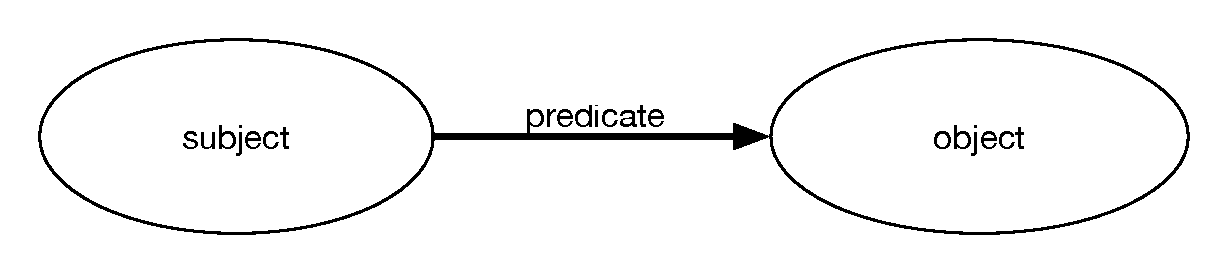
\includegraphics[width=0.75\linewidth]{images/rdf-graph}
	\caption{Semantic Web Stack} 
  	\label{fig:rdf-graph}
\end{figure}

A graphical representation of an RDF model is an RDF graph, where subjects and objects are nodes, while proprieties are represented as edges connecting a subject to an object, as can be seen in Figure \ref{fig:rdf-graph}


	



\subsection{Web Ontology Language}\label{sec:owl}
\subsection{Linked Data}\label{sec:ldata}
\subsection{SPARQL}\label{sec:sparql}


\section{Stream Processing}\label{sec:ifp}
\subsection*{Data Stream Management System}\label{sec:dsms}
\subsection{Complex Event Processor}\label{sec:cep}
\section{Stream Reasoning}\label{sec:sfp}
\subsection{RDF Stream Processing Engine}\label{sec:rspengine}
\section{Empirical Research}\label{sec:empirical-research}

The problem of understating the nature of the Computer Science (CS) research has one stronghold in Tichy's work of 1995 \cite{Tichy:1995:EEC:209090.209093}. He and his collaborator evaluated 400 articles published in 1993 randomly selected papers form ACM (50) and from a few journals in Systems and Software Engineering. The aim of Tichy's research was classify and define Computer Scientist research habits, proposing the following taxonomy, quoting from \cite{Tichy:1995:EEC:209090.209093}:
\begin{itemize}
\item \textit{Formal theory}: articles whose main contributions are formally tractable propositions, e.g., lemmata and theorems and their proofs.
\item \textit{Design and modelling}: systems, techniques, or models, whose claimed properties cannot be proven formally. Examples include software tools, performance prediction models, and complex hardware and software systems of all kinds. The papers in this class were further classified in the categories 0\%, 0–10\%, 10– 20\%, 20–50\, and +50\%, according to the proportion of the paper that was dedicated to the evaluation of the new system, technique, or model.
\item \textit{Empirical work}: articles that collect, analyse, and interpret observations about known designs, systems, or models, or about abstract theories or subjects (as this paper does). The emphasis is on evaluation, not on new designs or models.
\item \textit{Hypothesis testing}: articles that define hypotheses and describe experiments to test them.
\item \textit{Others}: articles that do not fit any of the four categories above, e.g., surveys.
\end{itemize}

Practically, an empirical study is just a test that compares what we believe to what we observe. The Testing activity, when properly designed and executed can be used to support the scientific method and rather plays a fundamental role in modern science. Empirical study helps us understand how and why things work, and allow us to use this understanding to materially alter our world.

Tichy's evaluation of paper from 1993 shows that despite the Engineering epistemology of the majority of the evaluated paper, there was a lack in empirical evaluation of the proposed research. More recent works \cite{Wainer:2009:EEC:1518331.1518552} observed confirmed Tichy's observations about the Computer Science engineering epistemology, the amount of evaluation reported in the papers is low.

The main reason for this is that software engineering (SE), and Computer Science, research has failed to produce the models and analytical tools that are common in other sciences \cite{Perry:2000:ESS:336512.336586}. CS research lacks the knowledge about the mechanisms which drive the costs and benefits of software tools and methods, making hard to understand whether analysis are  based on faulty assumptions or the new evaluation methods are properly.

Finally,  it is important to remember that empirical studies can be used not only retrospectively to validate systems or idea after they have been implemented, but also proactively to direct our research. Formal experiments, case studies and prototyping exercises are all adequate empirical studies. Independently from their form, they are a key way to fill the lack and sustains our research with credible observations. Indeed empirical studies allow to learn something useful by comparing theory to reality trough the following steps \cite{Perry:2000:ESS:336512.336586}:
\begin{itemize}
\item  formulating an hypothesis or question to test
\item  observing a situation
\item  abstracting observations into data
\item  analysing the data
\item  drawing conclusions with respect to the tested hypothesis
\end{itemize}


\section{Software Testing}
Software Testing (ST) techniques Starts with the intent of finding software bugs and ends with methods to evaluate system behaviour under testing conditions. In general software testing is an investigation over software products to evaluate the software quality. According to IEEE Standards  \cite{IEEEStd610.12-1990:glossary} there are two basic classes of software testing, black box testing and white box testing: 

\begin{itemize}
\item Black box testing [BBT] - it ignores the internal mechanisms of a system or component and focuses solely on the outputs
generated in response to selected inputs and execution conditions.
\item White box testing [WBT] - is takes into account the internal mechanism of a system or component. 
\end{itemize} 

Black-box testing  methods  examine the functionality of a system without peering into its internal structures or workings. BBT exploits test cases built around specifications and requirements of the software. An external descriptions of the software is mandatory, and it must also include software specifications, requirements and design parameters.  The test designer selects both valid and invalid inputs and determines the correct output without any knowledge of the test object's internal structure.

White-box testing  method instead exploits complete knowledge about software internal structures. In WBT an internal perspective of the system is required to design test cases. The test designer analyses the code, understand the expected output and chose input properly  to exercise paths he found. 

ST tries to offer an objective, independent view of the software, usually with Software Performance Testing, defined as  \textit{testing conducted to evaluate the compliance of a system or component with specified performance requirements} \cite{IEEEStd610.12-1990:glossary}. Once  the key transactions and their data requirements are identified, the test designer creates a number of different types of performance tests, in order to evaluate different software characteristics. The design of the test follows the researcher needs about which behaviour evaluate. The choice depends on the nature of the application and how much time is available for performance testing. The following testing terms are generally well known in the industry \cite{Molyneaux:2009:AAP:1550832}:

\begin{itemize}
\item \textit{Load testing} - it is the simplest form of performance testing, its aim is to understand the behaviour of the system under an expected load (the load kind depends on the software system) and meet performance targets for availability, concurrency or throughput, and response time. This test will give out the response times of all the critical transactions and it can point out bottlenecks in the application software. Load testing is the closest approximation of real application use.

\item \textit{Stress testing} -  it is used to understand the upper limits of capacity of a system and determine the system's robustness in terms of extreme load. A stress test may causes the application or some part of the supporting infrastructure to fail. The results of this kind of test are  capacity measure as much as performance. It's important to understand software limitations, in order to face future growth of application traffic, which may be hard to predict.

\item \textit{ Soak testing} - it is performed to determine if the system can sustain the continuous expected load. It essentially involves applying a significant load to a system for an significant period of time. The goal is to discover how the system behaves under sustained use or identify steady state conditions. During soak tests, memory utilization is monitored to detect potential leaks. Also important, but often overlooked is performance degradation, i.e. to ensure that the throughput and/or response times after some long period of sustained activity are as good as or better than at the beginning of the test. 
\end{itemize} 

\section{Benchmarks}
A benchmark is a procedure, problem, or test that can be used to compare systems or components to each other or to a standard \cite{IEEEStd610.12-1990:glossary}. Benchmarking is the primary method for measuring the performance of a systems, hardware or an application[7]. Benchmark results are used to evaluate the performance of a given system on a well-defined workload \cite{Menasce:2001:CPW:560806}.

Many benchmark tests exists to evaluate a wide variety system or applications under under different types of workloads. The user groups like the Transaction Processing Performance Council (TPC) \footnote{http://www.tpc.org/information},  a non-profit corporation founded to define transaction processing and database benchmarks, or analogues corporations are useful resources of be informed about updated types of benchmarks. 

Generic benchmarks allows the quantitative comparison of system performances or price/cost. In database context performance is typically a throughput metric (work/second) and price is typically a five-year cost-of-ownership metric. The quantitative comparison requires the benchmark to be run on several different systems and to record each system is measurements.  The estimation evaluated from results is usually the relative system performance, because the cost of implementing and measuring a specific application on many different systems is almost always prohibitive.

\subsection{Domain Specifc Benchmarks}  \label{sec:tcp}

A single metric can not measure the performance relative to all application of a computer systems \cite{DBLP:books/mk/Gray93}. Performances depend striclty on the application domain, because each system is designed for a few problem in a domain and may be inadequate to perform other tasks.

It is worth to note the work of Jim Gray about Domain-specific benchmarks, a kind of benchmarking methods and tools  which responds to computer system diversity. A Domain-specific benchmark specifies a synthetic workload characterizing typical applications in that problem domain. 

In order to distinguish among several solution and workload, Gray states four key criteria that a Domain-Specific Benchmark must meet to be useful\cite{DBLP:books/mk/Gray93}. It must be:
\begin{itemize}
\item Relevant: It must measure the peak performance and price/performance of systems when performing typical operations within that problem domain.
\item Portable: It should be easy to implement the benchmark on many different systems and architectures.
Gray: Introduction 3
\item Scalable: The benchmark should apply to small and large computer systems. It should be possible to scale the benchmark up to larger systems, and to parallel computer systems as computer performance and architecture evolve.
\item Simple: The benchmark must be understandable, otherwise it will lack credibility.
\end{itemize} 


\subsection{Reasoning Benchmark}\label{sec:lubm}

The number of different reasoners available is increasing and many of them are already commercial solutions. Usually reasoner are able to process very expressive ontology languages, which can represent rather complete knowledge, however there is an high demand of  less expressive ontology languages, which are less expensive in term of reasoning or other computational tasks. Commercial reasoner tries to solve the issue called \textit{computational cliff}, they face the trade-off between \textit{complexity and expressiveness} versus \textit{scalability}. Benchmarking tools are useful to evaluate reasoning system w.r.t. ontology languages 
\cite{bock2008benchmarking}. The most important Benchmark suite is the Lehigh University Benchmark  (LUBM) \cite{Guo2005}. This work proposes a  method for benchmarking Semantic Web knowledge base systems and provide an example of such a benchmarks.

Reasoning benchmarking environment requires:
\begin{itemize}
\item Ontology: LUBM exploits a synthetic ontology named Univ-Bench\footnote{http://www.lehigh.edu/~zhp2/2004/0401/univ-bench.owl} ,which describes universities, departments and the activities that occur at them. However, the popularity of OWL is high and that
many more ontologies are now available, and recent automated benchmarking tools allow testing performance with such ontologies\cite{gardiner2006automated}.

\item Workload: LUBM provides an random data generator, called UBA (Univ-Bench Artificial data generator), which creates extensional data over the Univ-Bench ontology \cite{Guo2005}.

\item Queries: LUBM comes with fourteen test queries to test the reasoning capabilities over the workload. LUBM method contains criteria for query definition which consider for example \textit{Input size} or \textit{Complexity} to stress the reasoner and evaluate performances.
\end{itemize}

Finally, Reasoning benchmarking require to understand which metrics evaluate such a system \cite{Guo2005}. LUBM contains three metrics which are commonly used in other database benchmarks.\begin{itemize}
\item \textit{Load Time,the stand alone elapsed time for storing the specified dataset to the system};
\item \textit{Repository Size, the resulting size of the repository after loading the specified benchmark data into the system};
\item \textit{Query Response Time}, as in databases benchmarking, for each test query the evaluation consist in:
  	1) Open the repository; 2) Execute the query for 10 times and compute the average response time. 3) Close the repository
\end{itemize}

LUBM contains also two specific reasoning metrics: \textit{Query Completeness and Soundness}: partial answering is possible in semantic web, indeed LUBM evaluate the \textit{degree of completeness of each query answer as the percentage of the entailed answers that are returned by the system is also evaluated}. Moreover, LUBM also provides a metric for measuring the combination of  query response time and answer completeness and soundness, to  appreciate the potential trade-off.

\subsection{DSMS \& CEP Benchmarking}\label{sec:linear-road}

Initial work on Streaming data like Linear Road \cite{arasu2004linear} firstly poses  several challenges to the design of a benchmark.  Moreover, the variety of CEP and DSMS domains and the lack of standards in query languages and data formats extends these benchmark design challenges. First of all DSMS Benchmarking must consider the challenges presented in the Linear Road work:
\begin{itemize}
\item  \textit{Semantically Valid Input} -  Input data can not be randomized but should have some semantic validity.
\item  \textit{Continuous Query Performance Metrics} - Standard DBMS time to completion metrics is inadequate. Query Response Time and Supported Query Load 
\item  \textit{Results Correctness} - benchmark implementations must be validated w.r.t the queries, which influence the results, to ensure that results are consistent with the benchmark specifications 
\item  \textit{Query Language Independence}: no standard query language for streaming systemsn exist, thus the query requirements must be language independent
\end{itemize}

Linear Road meets all the challenges above by design. The benchmark consist into a simulation of  an urban highways system where toll charges are dynamically determined. The Input data contains a stream of position reports, which specify the location of a vehicle every 30 seconds, and historical query requests, which may be issued by a vehicle with some fixed probability every time it emits a position report.

Further works, like the BiCEP project\footnote{http://bicep.dei.uc.pt} try to identify some o requirements for CEP benchmarking and develop a synthetic benchmarking set to measure the event processing activity such systems. CEP Benchmarking are evaluated with Jim Gray criteria presented in Section \ref{sec:tcp}. 

\begin{figure}[tbh]
  \centering
	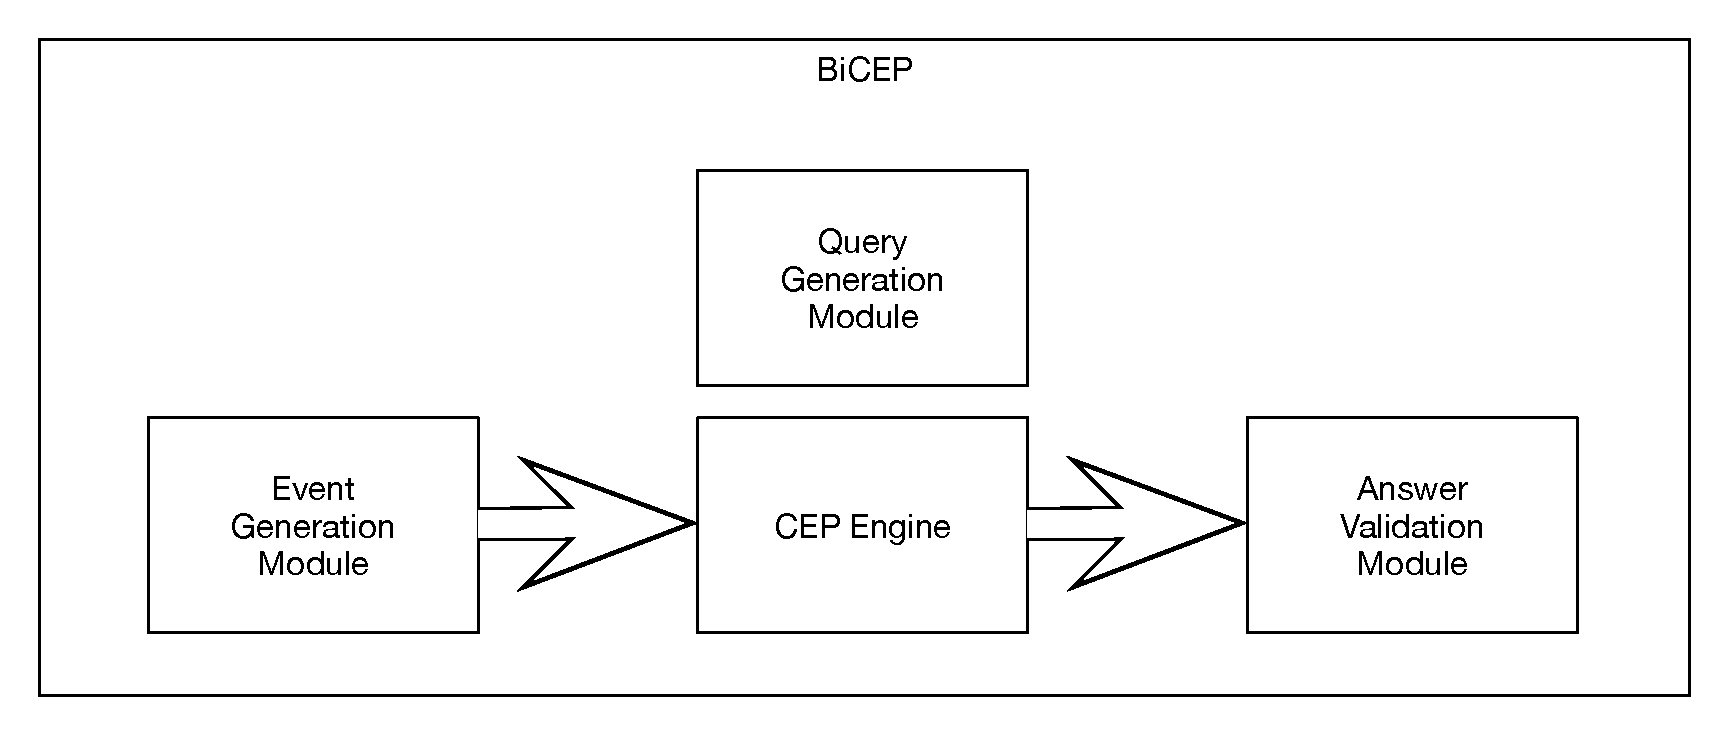
\includegraphics[width=\linewidth]{images/bicep_schema}
	\caption{BiCEP system  modules and the CEP engine} 
  	\label{fig:bicep-schema}
\end{figure}

BiCEP project also presents an first schema model for a benchmarking system, reported in Figure \ref{fig:bicep-schema}. The BiCEP benchmarking system will produce all the input trough the Event Generator Module, and consume the result output from the BiCEP CEP engine, with the Answer Validation Module. The Figure above also show how the CEP engine in interfaced with BiCEP modules, in order to ensure that any buffering, event cleaning or event transformation phase that happens at the CEP engine is part of the overall performance measure. Synthetic benchmarks offers many benefits like data availability, experimental control, and scalability. However, it is is hard to develop a synthetic benchmark that is representative of such a wide range of CEP applications and at the same time. BiCEP development is oriented towards a set of small domain specific synthetic benchmarks with different data sets and different queries \cite{bizarro:DSP:2007:1143}.

Finally, BiCEP project presents a set of metrics for CEP benchmarking, the most relevant ones in performance evaluation context are: \textit{Response time}: the time since the last event of some event pattern is fed into the system until the system notifies the event pattern detection. \textit{Scalability} in order to compare system with different scale levels; \textit{Adaptivity} the system response to input variation is mandatory, because CEP system rarely face stable input streams that allow the CEP engine to reach a steady state condition.



\subsection{Semantic Flow Processing (SFP) Benchmark}\label{sec:sr-benchmarking}

Section \ref{sec:empirical-research} shows how the empirical evaluation of system is increasing its relevance in the computer science context. SFP systems are complex and heterogeneous and this enforce the need of such empirical evaluation. However,  despite the increasing number of SFP engines, the works about SFP system evaluation are still limited and do not address proper definition of the key performance indicators (see Section \ref{sec:sfp}), making harder any comparison of  the different systems.

For this reason is worth to note the work on SFP benchmarking which was faced firstly the Challenges in this context (see Section \ref{sec:sfp}) by posing Seven commandments to follow on the benchmarking design \cite{DBLP:conf/esws/ScharrenbachUMVB13}:

Semantic Flow Processing engines must implement good \textit{Load Balancing} [S.1] strategies, because they usually consider several input information streams with possible bursts. It is possible to stress the system under various conditions by repeatedly applying a set of changes to the input and provide the empirical evaluation.

A stress test is required to measure the performance of \textit{Flow Data Joins And Inference} [S.2]. It has to consider increasingly complex cascades of joins in order to design the stress test for Simple joins, which put no further constraints on the join but the join-equality. The benchmark must have to add further constraints on the joins, and subsequently to  the data to enable testing Sequential joins, which add a sequential constrains, and Temporal joins, which extend sequential joins by enabling advanced temporal constraints. On the other and, \textit{joining stream and background data} [S.3] always results in simple joins. A stress-test must consider single joins and increasingly complex cascades.

The benchmark must test \textit{Aggregates} [S.4], which enable, on groups of entities or literals, counts, averages and any other arithmetic operation, trough properly scale groups: group number, group complexity or tuning the data to provide a big number of candidate but a small number of selected groups.

In distributed settings, SFP must ensure the correctness of query answers, handling \textit{Unexpected Data} [S.5] like out-of-order arrival of information and data loss.  A benchmark can measure this ability evaluating precision and recall of the amount of missing data with two tests, by increasing the number of out-of-order events (i) or by testing how long or how many data can be handled until some nosily data observation will be no longer considered for processing(ii).

A benchmarks has two possibility for stressing the system trough \textit{Schema} [S.6] variations: evaluating the system ability to handle an increasing number of of axioms in system ontology, notice that it is fundamental to add new axioms that could not have been deduced from existing ones. Changing statements that generate a more complex reasoning, it is important to know that increase the expressive power of the schema not only for the background data but also of the data flow may stress an SFP system significantly.

Finally, a benchmark should evaluate an SFP engine trough \textit{Changes in Background-Data} [S.7]. Any stress test on changes in background data should variate the update frequency and the entire amount of data involved in the update, forcing the system to access background-data from disk as much as possible.

Implemented proposal for SFP benchmarking has been published but none of them impact the community as the Linear Road did for DSMS. More careful analysis of those solutions evidence some lacks w.r.t proposed commandments \cite{DBLP:conf/esws/ScharrenbachUMVB13} 

\subsubsection{SRBench}\label{sec:srbench}

SRBench is presented as \textit{a general-purpose benchmark primarily designed for streaming RDF/SPARQL engines and based on real-world data sets}\cite{Zhang2012}. The SRBench dataset is composed by: the LinkedSensorData  which  is a real-world data set containing the US weather data published by Kno.e.sis\footnote{ http://knoesis.wright.edu};  GeoNames and DBpedia data sets, which allow to demostrate the ability of the benchmarked system to deal with interlinked data.

Moreover, \cite{Zhang2012} provides some relevant metrics to evaluate the performance of the system: \begin{itemize}
\item \textit{Correctness of the query results} - it must be validated and the validation results should be expressed in terms of precision and recall
\item \textit{Throughput} - it is defined as limit number of incoming data  an SFP system is able to process per time unit.
\item \textit{Scalability} - it means evaluating how the system reacts to an increasing number of incoming streams and variation on number of registered continuous queries.
\item \textit{Response time} - it is the amount of time between a data item enters the system and the SFP engine outputs the query results.
\end{itemize}

SR Bench provides also a query set composed by seventeen queries, which are designed based on a real use case in LSD. In order test many properties of the RDF stream engines the queries vary involving single or multiple input streams, queries over stream-only data sources or over mixed stream and static data source, etc. They cover the most important SPARQL operators and the common streaming SPARQL extensions and several queries require RDFS reasoning.

SRBench was criticised w.r.t. proposed commandments above \cite{DBLP:conf/esws/ScharrenbachUMVB13}. It only cover S.3, but the queries are fixed  and thus do not allow an exhaustive assessment of join performance, and S.6, thus testing variations of the expressive power is possible in SR but it was not done yet. Moreover, S.2 and S.4 are partially satisfied. The SRBench provides data and use-cases for sequential joins but it does not implement stress tests for temporal joins[S.2]. About S.4, SRBench  tests aggregates  by only implementing single queries. The other commandments are not cover yes, even if some of was marked as potential extensions of SRBench in \cite{DBLP:conf/esws/ScharrenbachUMVB13} Table 1.


\subsubsection{LSBench}\label{sec:lsbench}

LS Bench was developed to propose methods and a framework to enable  meaningful comparisons of SFP processing engines. The framework provides several customizable tools for simulating realistic data, running engines, and analysing the output. 

The LSBench proposed methods includes three tests to evaluate the SFP stream engines \cite{DBLP:conf/semweb/DellAglioCBCV13}. \begin{itemize}
\item A functional test to verify the operators and the functionalities supported
by the engines, similar to SR Bench \ref{sec:srbench}
\item A correctness test is to verify if the tested SFP engine produces the correct output. Actually the test assumes that the contents of the output are correct, and it analyses only the number of produced answers.
\item A maximum input throughput test, whose aim is evaluating the maximum throughput of the SFP engine, by increasing the data streak rate and checking the number of the answers
\end{itemize}

%\subsubsection{LSBench} S2 partially, S3 partially, S4 partially 

The data generator, S2Gen, creates data set for benchmarking according to the \textit{Social Network Data Stream Logic Schema} presented in \cite{LePhuoc2012c} Figure 1. S2Gen allow to tune three parameters which influence the data generation task: 1) \textit{Generating period}, the period in which the social activities are generated; 2) Maximum number of posts/comments/photos for each user per week 3) the \textit{Correlation probabilities}: there are various parameters for the data correlations which can be customized to specify how data is related according to each data attribute.

Finally, LSBench \cite{LePhuoc2012c} provides for each test a set of 12 fixed queries. The queries in the set vary to address different features of the engines. In relation with the Seven commandments for SFP benchmarking, not all of the are covered by LS Bench \cite{DBLP:conf/esws/ScharrenbachUMVB13} Table 1. LSBench cover S3, like SRBench fixed queries do not allow to stress the system properly with the aim of evaluate join performances. S2 is only partially supported, because, like SRBench, LS Bench does not support stress testing for temporal joins but only for sequential. S4 is again only partially fulfilled: LS Bench test aggregates only implementing single queries  \cite{DBLP:conf/esws/ScharrenbachUMVB13}.


%\subsubsection{Correttezza}
%\subsubsection{Seven Commandaments}

